\documentclass[border=10pt]{standalone}
\usepackage{tikz}

\tikzstyle{vertex}=[circle,draw,fill=black!20,minimum size=0.7cm,inner sep=0pt]
\tikzstyle{selected vertex} = [vertex, fill=red!24]
\tikzstyle{edge} = [draw,thick,-]
\tikzstyle{weight} = [font=\small]
\tikzstyle{selected edge} = [draw,line width=5pt,-,red!50]
\tikzstyle{ignored edge} = [draw,line width=5pt,-,black!20]

\begin{document}
\noindent
    \centering
    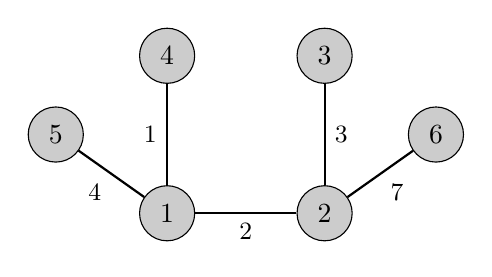
\begin{tikzpicture}[scale=1.0,transform shape,auto,swap]
        \node[vertex] (1) at (0, 0) {1};
        \node[vertex] (2) at (2, 0) {2};
        \node[vertex] (3) at (2, 2) {3};
        \node[vertex] (4) at (0, 2) {4};
        \node[vertex] (5) at (-1.414, 1) {5};
        \node[vertex] (6) at (3.414, 1) {6};
        \path[edge] (1) -- node[weight] {2} (2);
        \path[edge] (2) -- node[weight] {3} (3);
        \path[edge] (4) -- node[weight] {1} (1);
        \path[edge] (1) -- node[weight,below left] {4} (5);
        \path[edge] (2) -- node[weight] {7} (6);
    \end{tikzpicture}
\end{document}
